Leonardo, like many other Italian scientists and artists of his age, was extremely interested in city planning and urban design. He aimed to model an ideal city: comfortable, spacious and rational in its usage of resources, far away from the narrow, claustrophobic cities of the Middle Ages.

\bf{The ideal city}

The city is made of $N$ blocks placed on an infinite grid of cells. Each cell is identified by a pair of coordinates (row, column). Given a cell $(i, j)$, the adjacent cells are: $(i - 1, j)$, $(i + 1, j)$, $(i, j - 1)$, and $(i, j + 1)$. Each block, when placed onto the grid, covers exactly one of the cells. A block can be placed onto the cell $(i, j)$ if and only if $1 \le i, j \le 2^{31} - 2$. We will use the coordinates of the cells to also refer to the blocks on top of them. Two blocks are adjacent if they are placed in adjacent cells. In an ideal city, all of its blocks are connected in such a way that there are no ``holes'' inside its border, that is, the cells must satisfy both conditions below.

\begin{itemize}
\item For any two empty cells, there exists at least one sequence of adjacent empty cells connecting them.
\item For any two non-empty cells, there exists at least one sequence of adjacent non-empty cells connecting them.
\end{itemize}

\bf{Example 1}

None of the configurations of blocks below represent an ideal city: the first two on the left do not satisfy the first condition, the third one does not satisfy the second condition, and the fourth one does not satisfy either of the conditions. 

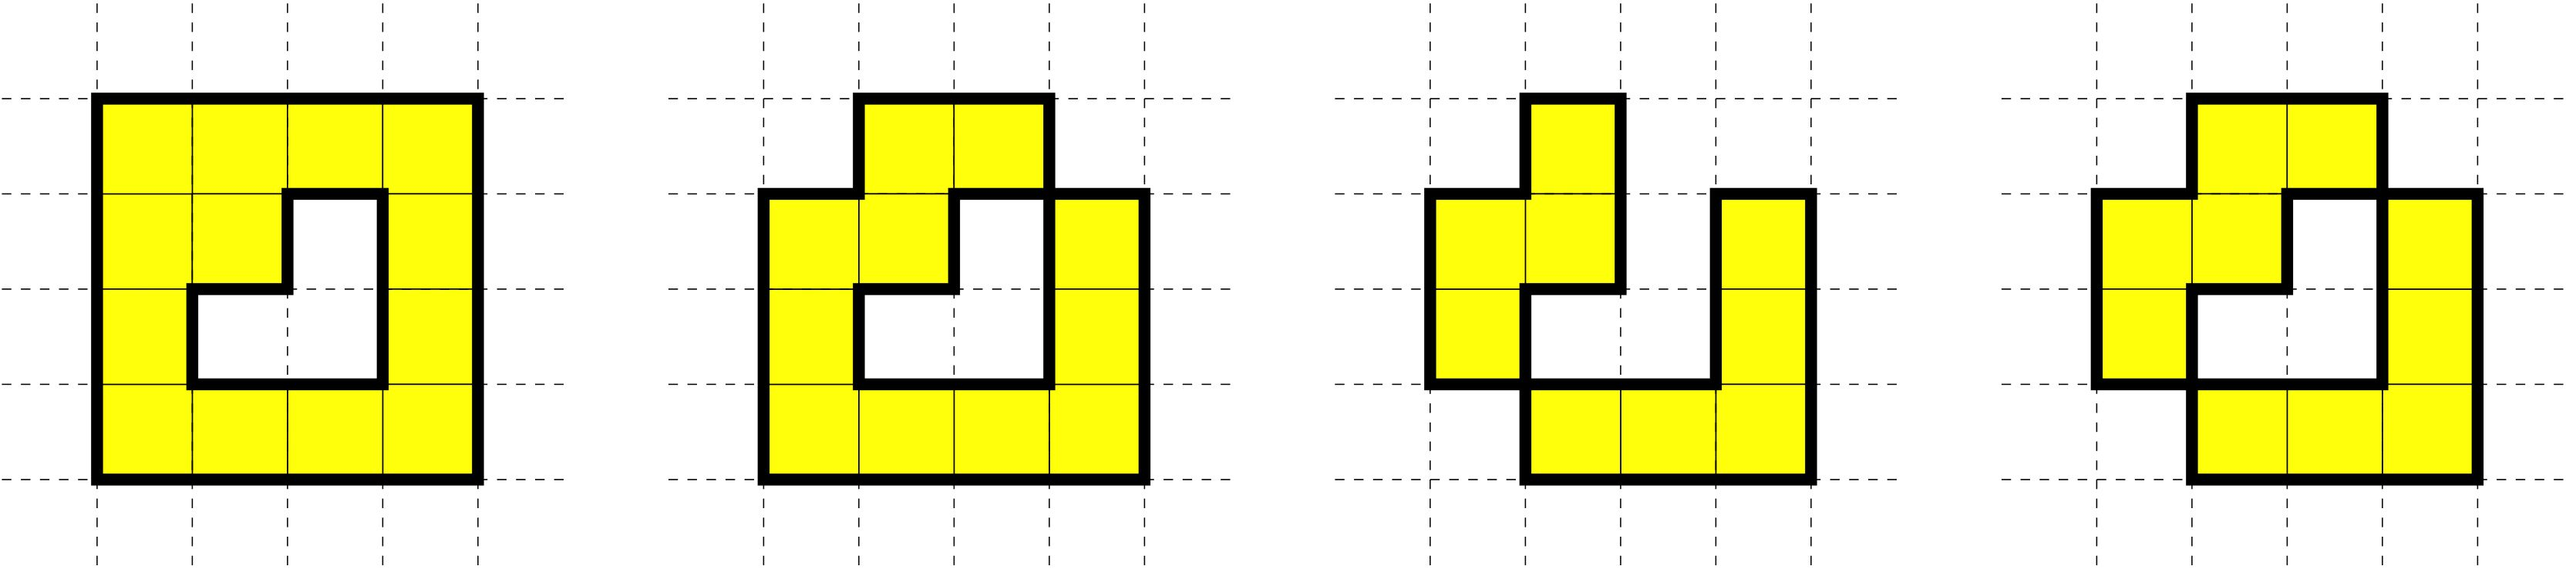
\includegraphics{2012-4-01.jpg}

\bf{Distance}

When traversing the city, a hop indicates going from one block to an adjacent one. Empty cells cannot be traversed. Let $v_0, v_1, \dots, v_N$ be the coordinates of the N blocks placed on the grid. For any two distinct blocks at coordinates $v_i$ and $v_j$, their distance $d(v_i, v_j)$ is the smallest number of hops that are required to go from one of these blocks to the other one.

\bf{Example 2}

The configuration below represents an ideal city made of $N = 11$ blocks.

\begin{tabular}{crcl}
\multirow{10}{*}{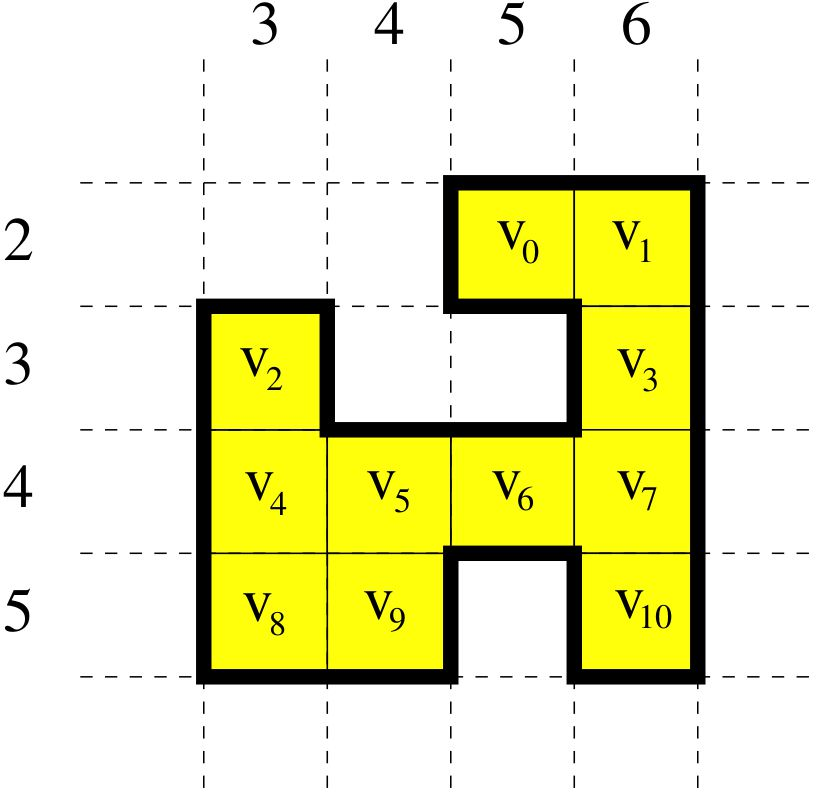
\includegraphics[height = 27ex]{2012-4-02.jpg}}& 
$v_0$ &$=$& $(2,5)$\\
&$v_1$ &$=$& $(2,6)$\\
&$v_2$ &$=$& $(3,3)$\\
&$v_3$ &$=$& $(3,6)$\\
&$v_4$ &$=$& $(4,3)$\\
&$v_5$ &$=$& $(4,4)$\\
&$v_6$ &$=$& $(4,5)$\\
&$v_7$ &$=$& $(4,6)$\\
&$v_8$ &$=$& $(5,3)$\\
&$v_9$ &$=$& $(5,4)$\\
&$v_{10}$ &$=$& $(5,6)$\\
\end{tabular}

For example, $d(v_1, v_3) = 1$; $d(v_1, v_8) = 6$; and $d(v_9, v_{10}) = 4$.

\bf{Statement}

Your task is to, given an ideal city, write a program to compute the sum of all pairwise distances between blocks $v_i$ and $v_j$ for which $i < j$. Formally, your program should compute the value of the following sum: 

\begin{center}
$\sum d(v_i, v_j)$; where $0 \le i < j \le N-1$
\end{center}

Specifically, you have to implement a routine \t{DistanceSum(N, X, Y)} that, given $N$ and two arrays $X$ and $Y$ that describe the city, calculates the formula above. Both $X$ and $Y$ are of size $N$; block $i$ is at coordinates $(X[i], Y[i])$ for $0 \le i \le N - 1$, and $1 \le X[i], Y[i] \le 2^{31} - 2$. Since the result may be too big to be represented using 32 bits, you should report it modulo $1\,000\,000\,000$ (one billion). In Example 2, there are $\frac{11 × 10}{2} = 55$ pairs of blocks. The sum of all the pairwise distances is $174$.

\bf{Implementation details}

You have to submit exactly one file, called \t{city.c}, \t{city.cpp} or \t{city.pas}. This file must implement the subprogram described above using the following signatures.

This subprogram must behave as described above. Of course you are free to implement other subprograms for its internal use. Your submissions must not interact in any way with standard input/output, nor with any other file.

\bf{Sample grader}

The sample grader provided with the task environment will expect input in the following format:

\begin{itemize}
\item line 1: $N$;
\item lines 2, \ldots, N + 1: $X[i]$, $Y[i]$.
\end{itemize}

